\chapter{Experimental Setup}
This chapter provides a detailed overview of the experimental setup used in this research, ensuring transparency and reproducibility of the results. The chapter begins with Section \ref{sec:hardware}, which outlines the hardware configuration, describing the computational resources such as \glspl{cpu}, \glspl{gpu}, and storage systems utilized during the experiments. Section \ref{sec:software} follows with a description of the software environment, detailing the programming languages, libraries, and tools employed.

Next, Section \ref{sec:data} introduces the datasets used in this study, focusing on the \gls{nba} and \gls{dfl} datasets. This section includes a discussion of the specific data preprocessing steps required to prepare the data for analysis, including data transformation and normalization techniques. The detailed description of the dataset structures, provided in Sections \ref{sect:NBA} and \ref{sect:SOC}, ensures that the data used in the experiments can be accurately replicated and extended in future research.

Section \ref{sec:experiments} outlines the experimental procedures conducted to evaluate the performance of different predictive models. This includes an exploration of various factors such as input data types (positional versus velocity data), the effect of historical context and forecast horizons, and comparisons between univariate and multivariate prediction models. The section also covers intra-team versus inter-team performance evaluations and the impact of transfer learning across different domains.

Finally, Section \ref{sec:model_configs} describes the specific model configurations used in the experiments. This includes linear models, \gls{lstm} networks, \gls{lmu} models, Transformer models, and BitNet models. Each model's architecture is discussed in detail, with explanations of how they process the input data and generate predictions. The chapter concludes with a summary of how these configurations were used to comprehensively evaluate the models' capabilities across different experimental conditions.


\section{Hardware Configuration}
\label{sec:hardware}
The computational experiments were conducted on a high-performance cluster running CentOS Linux 7.9.2009 with kernel version 3.10.0-1160.71.1. The cluster consists of 8 \gls{gpu} nodes and 4 \gls{cpu} nodes. Each \gls{cpu} node is equipped with two Intel Xeon Gold 5120 processors, each featuring 28 cores and 2 threads per core, operating at a base frequency of 2.20 GHz. Each \gls{gpu} node contains two Intel Xeon Gold 5120 processors and four Tesla V100-SXM2 \glspl{gpu}, each with 32,768 MiB of dedicated memory.

\section{Software Configuration}
\label{sec:software}

This research employs Conda (version 23.10.0) as a crucial tool for managing software environments and dependencies. Conda simplifies the installation of required libraries, ensuring compatibility across a variety of computational tasks. The programming language Python (version 3.11.0) serves as the foundation for developing, testing, and benchmarking the machine learning models used in this study.

The \texttt{pyproject.toml} file for Gosalci's project \cite{Gosalci_master_den_2024} defines the essential Python packages needed for the project. These include \texttt{torch==2.4.1+cu118} for deep learning applications with CUDA support (version 11.8), \texttt{numpy==2.0.1} for efficient numerical operations, \texttt{pandas==2.2.2} for data processing and manipulation, \texttt{matplotlib==3.9.1.post1} for data visualization, \texttt{scipy==1.14.0} for scientific computing tasks, \texttt{Pillow==10.4.0} for image processing, \texttt{py7zr==0.21.1} for handling 7z archives, \texttt{codecarbon==2.5.1} for tracking carbon emissions from computations, \texttt{lightning==2.4.0} for managing PyTorch Lightning models, \texttt{tensorboard==2.17.1} for monitoring training metrics, \texttt{wandb==0.17.7} for experiment tracking and visualization, and \texttt{pip==24.2} for managing additional Python packages. Together, these tools are fundamental to running the complex computational workflows outlined in this thesis. Installation and execution instructions can be found in the \texttt{README.rft} file within the same project.

Local development is conducted using VSCodium and PyCharm on a Windows 10.0 host machine. These \glspl{ide} allow for efficient code writing and debugging, while computation-heavy tasks are offloaded to the high-performance cluster.



\section{Datasets}
\label{sec:data}

This chapter presents the datasets employed for developing and assessing predictive models for player and ball movements in basketball and soccer. The first dataset, described in Section \ref{sect:NBA}, comes from the \gls{nba} and captures player interactions on a uniform court. This dataset supports accurate model development thanks to the consistent court dimensions. The second dataset, detailed in Section \ref{sect:SOC}, covers soccer and includes data from various field sizes and player tactics, adding complexity to the analysis. Both datasets provide detailed positional and velocity information recorded at high frequencies. They were preprocessed for consistency and reliability, facilitating effective model training and comparison. The following sections offer a detailed look at each dataset and the preprocessing methods used.

\subsection{NBA}
\label{sect:NBA}
The \gls{nba} is a fast-paced and highly dynamic sport where players regularly demonstrate rapid bursts of speed, sharp directional changes, and explosive movements. The game is characterized by quick transitions between offense and defense, frequent sprints across the court, and an ever-evolving gameplay that demands both physical agility and mental adaptability. The court is strictly regulated, measuring 28.65 meters in length and 15.24 meters in width, providing a uniform environment for analysis (see Figure \ref{fig:nba_court}). These dimensions contrast with sports like soccer described in Section \ref{sect:SOC}, where the field size can vary between datasets. The fixed court size in basketball ensures that the spatial metrics are consistent across different games, allowing for more precise modeling. These factors, combined with the high intensity of player interactions, create a competitive environment where outcomes are difficult to predict, even for seasoned experts. This inherent unpredictability underscores the necessity for the advanced models detailed in Chapter \ref{chapt:method}.

\begin{figure}[t]
    \centering
    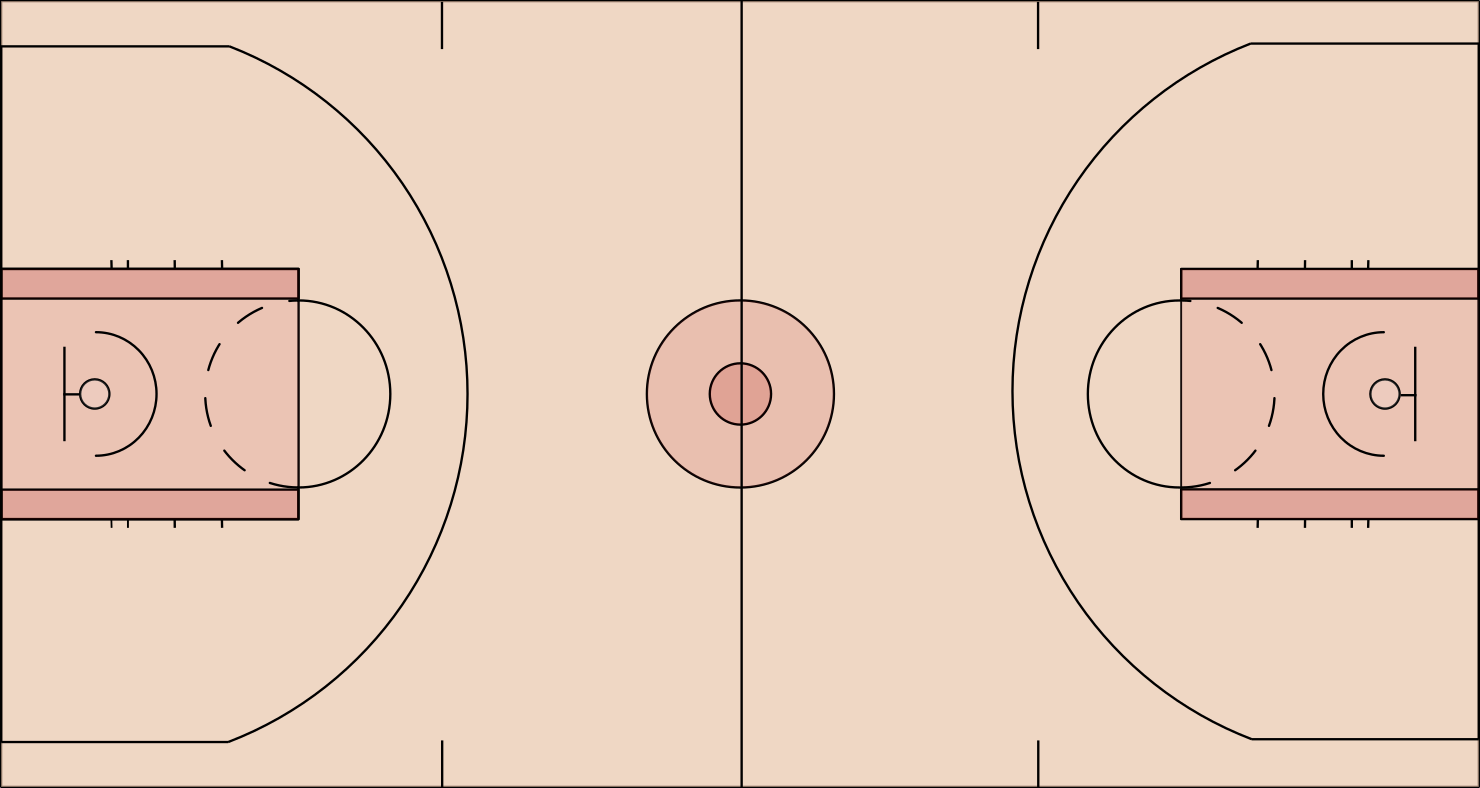
\includegraphics[width=\textwidth]{contents/nba_court.png}
    \caption{Diagram of an NBA court.}
    \label{fig:nba_court}
\end{figure}

\subsubsection{structure overview}
\label{sect:original_nba}

To facilitate the development and validation of these models, this study utilizes a dataset sourced from the ``NBA-Player-Movements'' repository by Linou et al. \cite{linouk}. The dataset contains 636 games from the 2015/16 season. Each game is stored in a compressed ``.7z'' format, which can be extracted using tools such as 7zip. Once extracted, the data is presented in a ``.json'' format, which was further processed using Python to prepare it for analysis.

Upon reading the JSON file into a pandas DataFrame, the data is structured with three primary columns: \textbf{``gameid''}, \textbf{``gamedate''}, and \textbf{``events''}. The \textbf{``gameid''} and \textbf{``gamedate''} columns contain the unique identifier for each game and the corresponding date, respectively. These values remain constant for each row (event) within a single game. The \textbf{``events''} column contains detailed information about each individual event, represented as a dictionary. The keys of this dictionary are \textbf{``eventId''}, \textbf{``visitor''}, \textbf{``home''}, and \textbf{``moments''}. Information regarding the \textbf{``visitor''} and \textbf{``home''} keys, which provide details about the teams involved, is discussed in Section \ref{sect:teams}. Details about the \textbf{``moments''} key, which contains information on specific moments within events, will be elaborated on in Section \ref{sect:moments}.

Figure \ref{fig:data-structure} provides a graphical representation of the dataset structure, illustrating the organization of the data columns and the relationships between different elements, including the main file structure, team details, and moment details.

\subsubsection{Home and Visitor Team}
\label{sect:teams}

In the dataset, information about both the home and visitor teams is provided under the \textbf{``home''} and \textbf{``visitor''} keys, respectively. Each team is represented as a dictionary that contains several important details. Specifically, the dictionary includes the team's \textbf{``name''}, which is its official designation, the \textbf{``teamid''}, a unique identifier used to distinguish the team from others, and the \textbf{``abbreviation''}, which is a short code representing the team’s name for convenience.

Within each team dictionary, there is a \textbf{``players''} key that points to a list of dictionaries. Each dictionary in this list represents an individual player on the team. For each player, the dictionary includes the \textbf{``lastname''} and \textbf{``firstname''}, which together identify the player. It also includes the \textbf{``playerid''}, a unique identifier for the player, and the \textbf{``jersey''} number, which is unique within the team and indicates the player's number. Lastly, the \textbf{``position''} describes the player’s role on the team, such as forward, center, or guard. Figure \ref{fig:data-structure} shows the structure graphically. 

\subsubsection{Moments}
\label{sect:moments}

The \textbf{``moments''} key in the dataset provides detailed information about specific events within the game. Each entry under this key is a list of \textbf{``moment''}s, where each \textbf{``moment''} contains several pieces of information. These details include the \textbf{``quarter''}, which indicates the quarter number during which the moment occurred, and the \textbf{``moment\_id''}, representing the absolute timestamp of the moment in UNIX format. Additionally, \textbf{``game\_clock''} and \textbf{``shot\_clock''} provide further temporal information, measured in seconds. The \textbf{``None''} field typically remains empty and does not contain any data.

The \textbf{``objects''} key within each moment lists the details of all players on the field and the ball, usually totaling 11 entries: 5 players from each team and the ball. For each entry, the data includes \textbf{``teamid''} and \textbf{``playerid''}, which are consistent across all moments. Additionally, \textbf{``x\_pos''} and \textbf{``y\_pos''} provide the positional information of each player in feet, with the origin defined as the lower left corner of the field. The \textbf{``ball\_radius''} is relevant only for the ball, providing its radius, which indirectly gives information about the ball's height or z-axis position. For a visual representation of the structure of these moment details, please refer to Figure \ref{fig:data-structure}.

\begin{figure}[t]
\centering
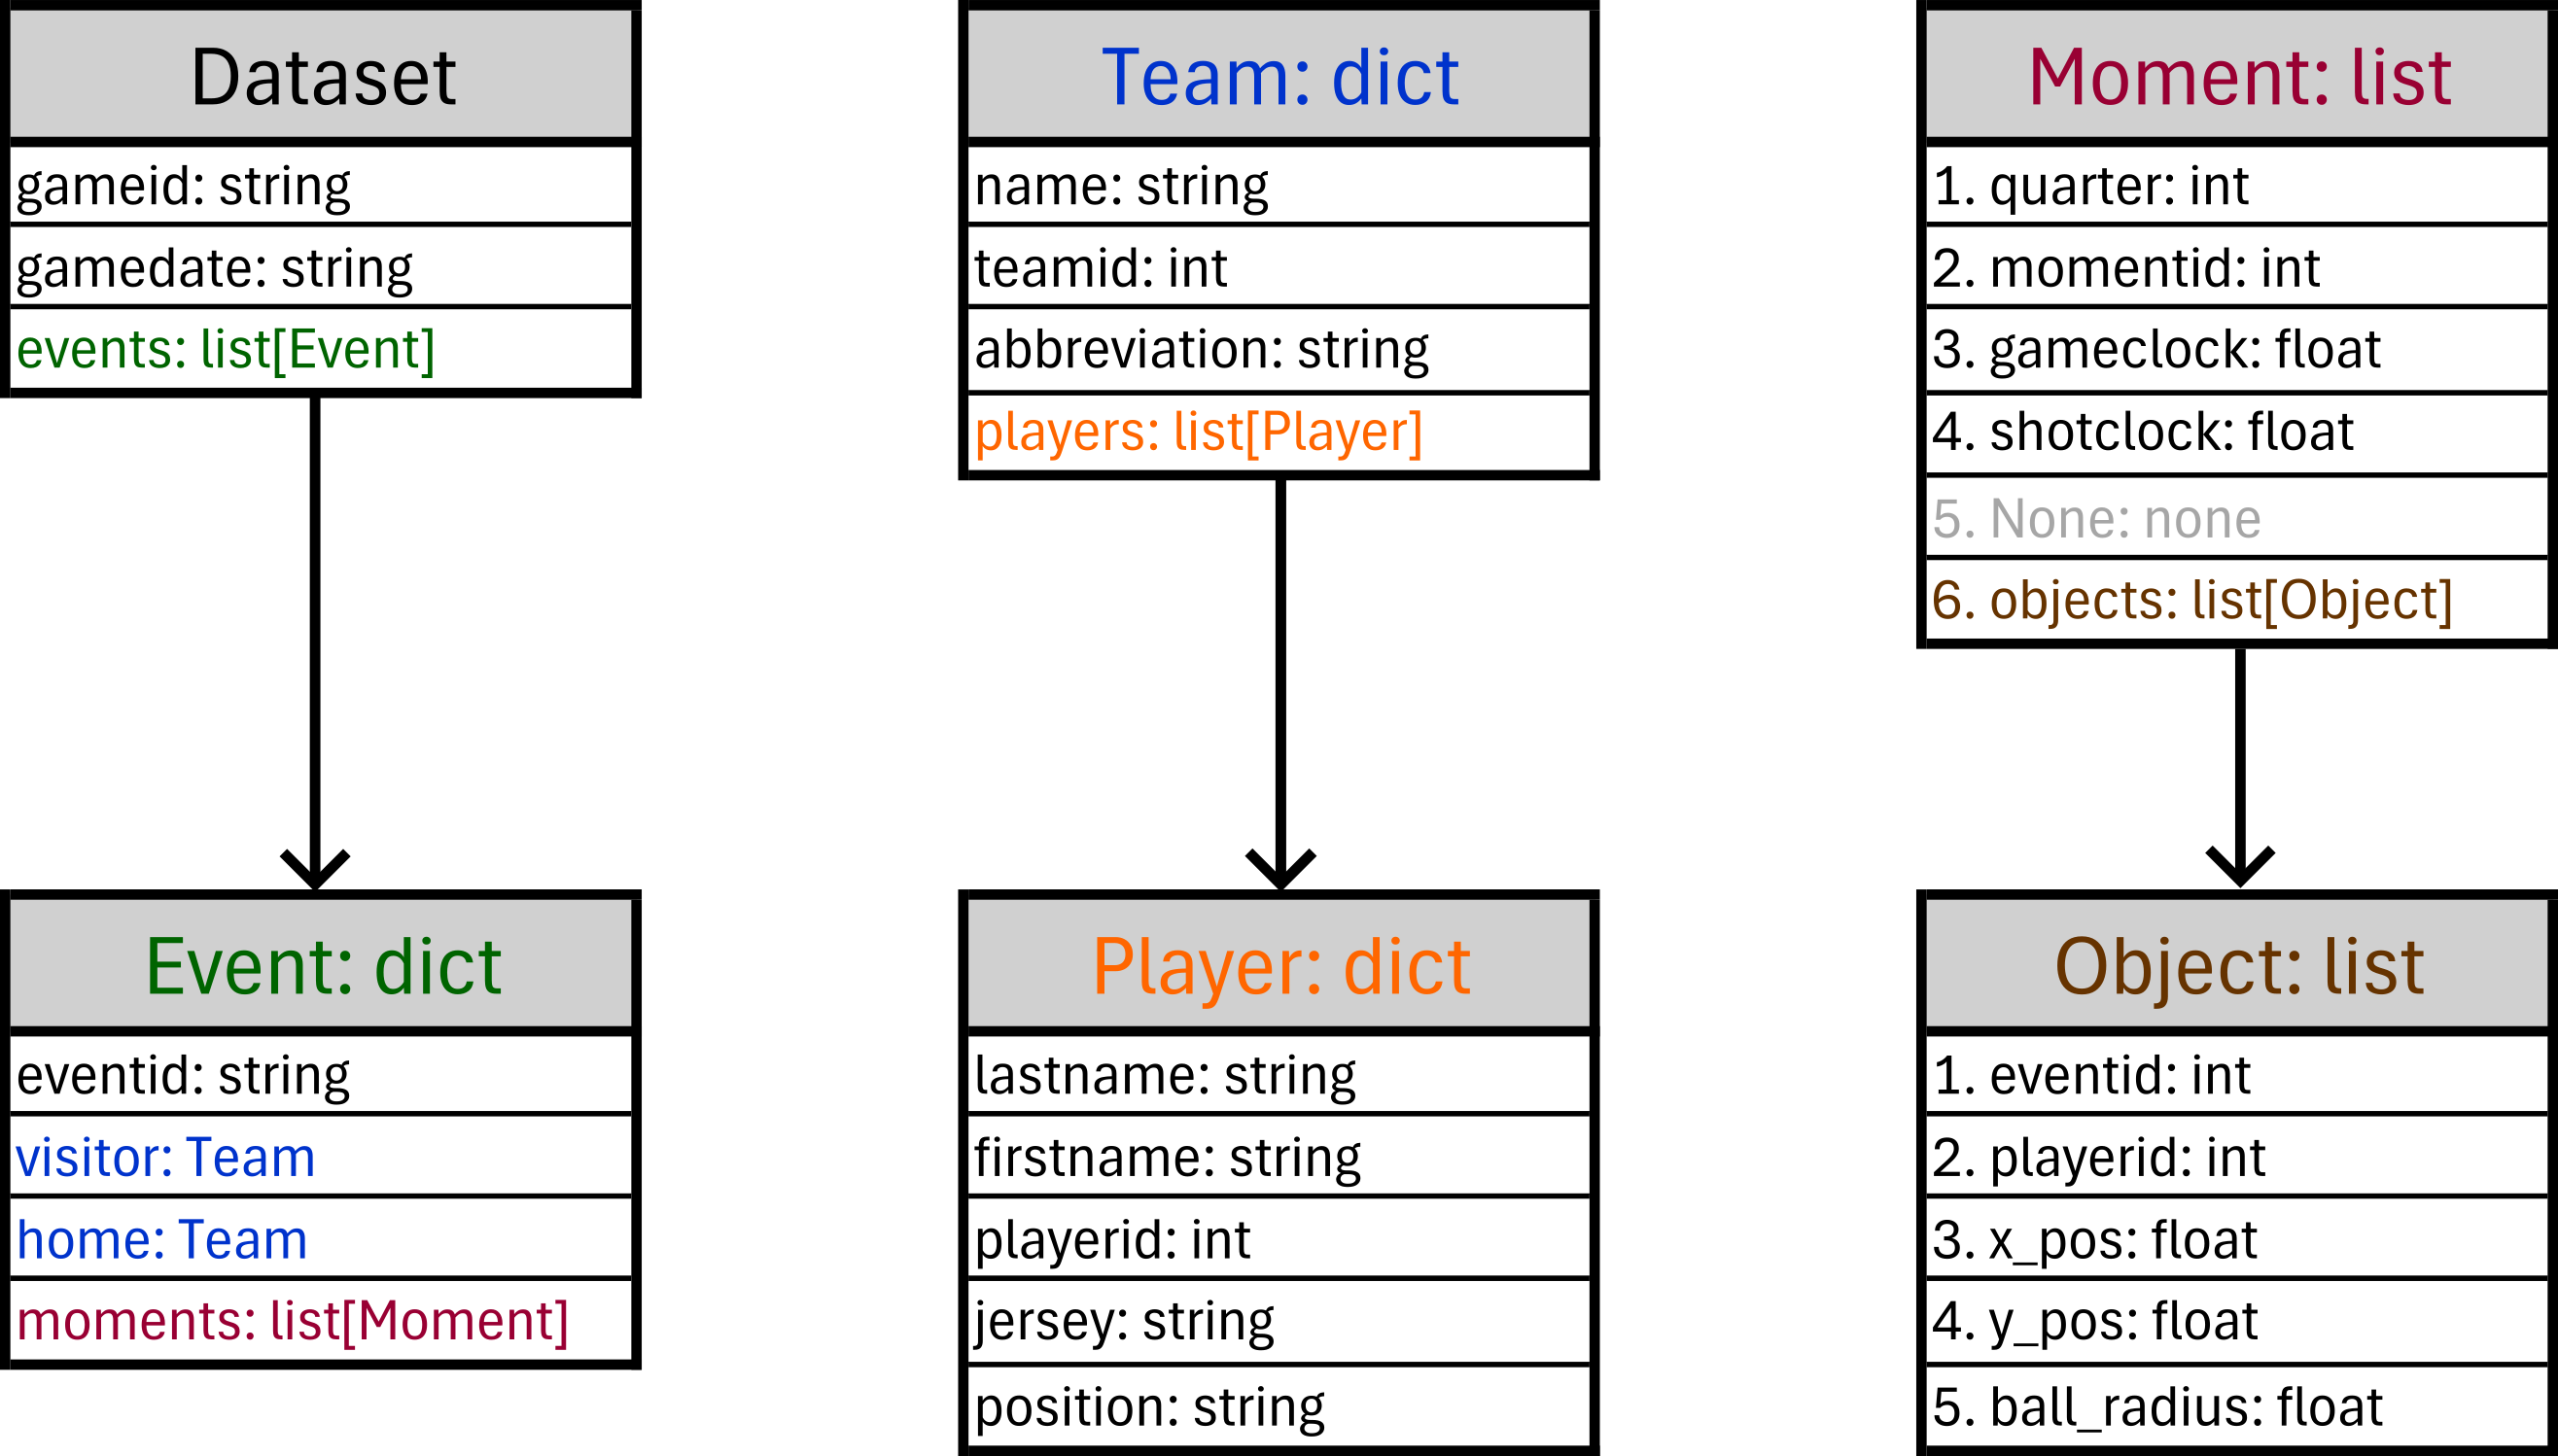
\includegraphics[width=\textwidth]{contents/data-structure.png}
\caption{Graphical representation of the dataset structure, including the main file (left) and details about the home and vistor teams (center), and moments (right).}
\label{fig:data-structure}
\end{figure}


\subsubsection{Data Preparation and Transformation}
\label{sect:data-prep}

To create a usable dataset, several preparation steps were undertaken. The complex nested structure described earlier was simplified into a more manageable two-dimensional DataFrame. Each moment was converted into a row, with all relevant information contained within these rows. While this transformation increased disk usage due to the replication of data, such as game dates and game IDs, which were previously represented only once per match, the trade-off was justified by the improved accessibility and ease of use gained through flattening the structure.

Each moment contains data for 11 objects—comprising 5 players from each team and the ball—each with distinct attributes like position and velocity. To streamline the dataset, unnecessary fields were removed, including \textbf{``firstname''}, \textbf{``lastname''}, \textbf{``jersey''}, \textbf{``teamname''}, \textbf{``gamedate''}, and irrelevant fields such as the \textbf{``None''} column. This decision was based on the focus of the task, which required generalizable models rather than identification of individual players or teams. By retaining only the essential data, such as the game name in the filename and removing these extraneous columns, disk space usage was reduced by precisely \(62.30\%\).

The resulting dataset contains, for each moment, the positions (\textbf{x\_pos}, \textbf{y\_pos}) and velocities (\textbf{vx}, \textbf{vy}) of all 10 players and the ball. These positions are specified in feet, with the origin defined at the lower left corner of the court. The velocity data is derived from the positional changes over time and provides crucial information for dynamic analysis.

The original dataset was recorded primarily in 0.04-second intervals, equating to a sampling rate of 25Hz. However, due to occasional missing data points, some time spans were incomplete. To ensure consistency and maintain the temporal resolution, these gaps were filled using interpolation. Missing values were interpolated to preserve the integrity of the time series data, enabling a seamless analysis of player and ball movements. 

To further enhance consistency, the rows were sorted by ascending event numbers and then by \textbf{``moment\_id''} within each event. Additionally, events with fewer than 8 seconds of data (or fewer than 200 \textbf{``moments''}) were excluded to maintain consistency across the dataset and reduce the risk of bias from shorter events, which are typically not useful for many models. After cleaning, the dataset shrank by 36.44\%, resulting in approximately 163,000 remaining events.

The overall reduction in data size, considering both row and column cleaning, was calculated as \(z = 1 - (1 - x)(1 - y) = 1 - (1 - 0.623)(1 - 0.3644) \approx 0.76\). This indicates that more than three-quarters of the original data was ultimately removed during preprocessing. The final dataset is a single two-dimensional DataFrame consisting solely of the unique \textbf{event\_id}, unique \textbf{moment\_id}, and the positions and velocities of all players and the ball.

To prepare the data for model training, the dataset was split into training and validation sets using a 90-10 ratio. All games were included in these sets except for one specific game, \textbf{TOR@LAL}, where \textbf{TOR} is the visiting team and \textbf{LAL} is the home team. This particular game was set aside as the testing dataset. The model was initially trained exclusively on data from the Lakers to investigate its adaptability when applied to a different team, which serves as the focus of the research question. This approach allows for an examination of how well the model generalizes from one team to another, providing insights into its performance and adaptability in various contexts.


\textbf{Velocity Calculation for Each Time Step:}  
To compute the velocity from the positional data provided in the \textbf{``x\_pos''} and \textbf{``y\_pos''} fields at each moment, three differentiation methods are employed, depending on the time step. Special cases are required for the first and last time steps due to the lack of neighboring data points at these boundaries. The calculated velocities are saved as \textbf{``x\_vel''} and \textbf{``y\_vel''} alongside with the index of the player:

\begin{itemize}
    \item \textbf{First Time Step (Forward Differentiation):} For the first time step, velocity is approximated using forward differentiation:
    \[
    v(t_0) = \frac{x(t_1) - x(t_0)}{\Delta t}
    \]
    This method is used because there is no preceding time step to use for backward differentiation.

    \item \textbf{Intermediate Time Steps (Central Differentiation):} For all intermediate time steps (excluding the first and last), velocity is calculated using central differentiation:
    \[
    v(t_i) = \frac{x(t_{i+1}) - x(t_{i-1})}{2 \Delta t}
    \]
    This method provides a more accurate approximation of velocity at each intermediate time step \( t_i \) by utilizing both neighboring points.

    \item \textbf{Last Time Step (Backward Differentiation):} At the final time step, velocity is estimated using backward differentiation:
    \[
    v(t_n) = \frac{x(t_n) - x(t_{n-1})}{\Delta t}
    \]
    This approach is used due to the lack of subsequent data points needed for forward differentiation.
\end{itemize}


\subsection{Soccer}
\label{sect:SOC}
Soccer, like basketball, is a dynamic and fast-paced sport where two teams compete to control the ball and score goals. Both sports emphasize teamwork, strategy, and quick decision-making, making them useful for testing similar predictive models. However, a key difference lies in the playing field. Unlike the strictly regulated NBA court, which measures approximately 28.65 meters in length and 15.24 meters in width, soccer fields are not uniformly sized across all datasets or competitions. The size of a soccer field can vary significantly, typically ranging between 100-110 meters in length and 64-75 meters in width. This variability in field dimensions can introduce additional complexity when processing soccer data for comparison with basketball data.

To address this, it is crucial to normalize the soccer dataset into the same format as the NBA dataset \ref{sect:NBA} for consistency in analysis and accurate comparison between the two sports. The soccer court dimensions used in this dataset are illustrated in Figure \ref{fig:soccer_court}, which provides a visual representation of the standard field layout and dimensions.

\begin{figure}[t]
    \centering
    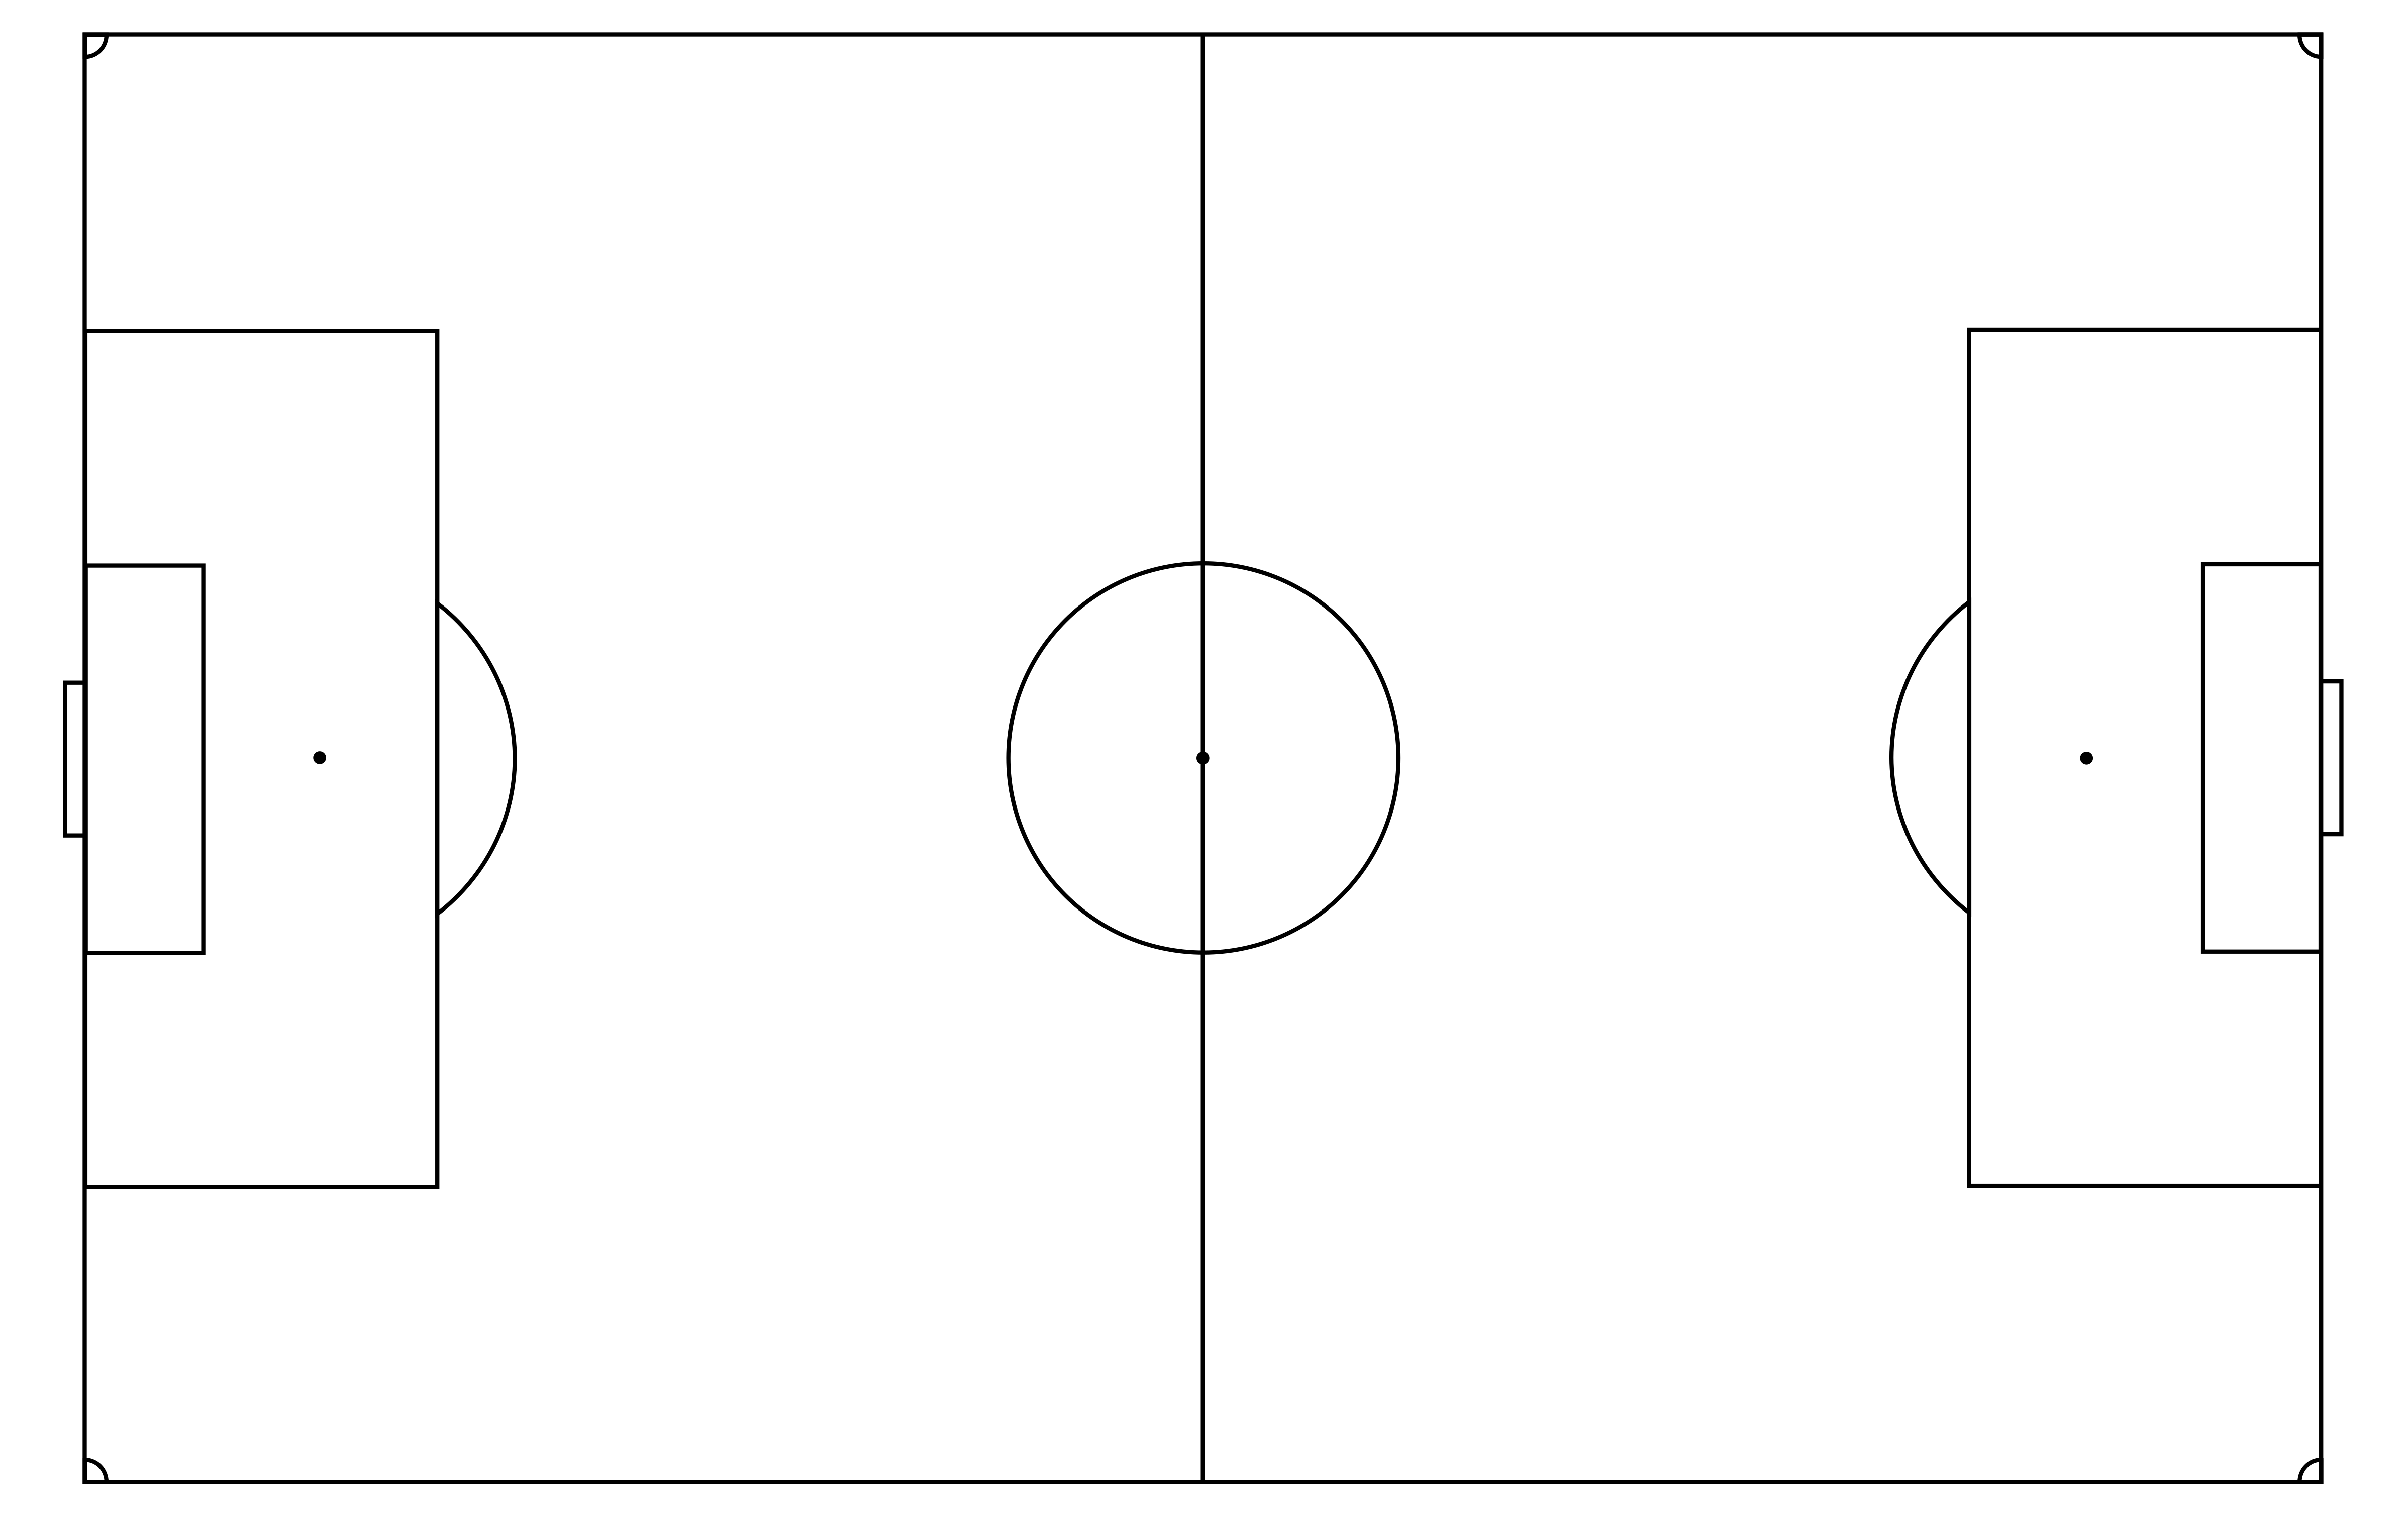
\includegraphics[width=\textwidth]{contents/drawing_rg.png}
    \caption{Diagram of a soccer field.}
    \label{fig:soccer_court}
\end{figure}



\subsubsection{structure overview}
\label{soc:details}
The Soccer dataset consists of 316 games from the Deutsche Fu{\ss}ball Liga (DFL) for the 2014/15 and 2015/16 seasons and was provided by the Fraunhofer Institute for Integrated Circuits IIS. Unlike the original NBA files, the Soccer dataset is flat and straightforward. It is organized into two separate two-dimensional datasets: one for the ball \ref{sect:ball} and one for the players \ref{sect:players}. In this dataset, information about players, teams, and games is replaced with encrypted text to ensure privacy and anonymity.

\subsubsection{Ball}
\label{sect:ball}

The dataset also includes detailed information about the ball at every moment during the game. The relevant fields are \textbf{BallStatus}, \textbf{M}, \textbf{N}, \textbf{Period}, \textbf{S}, \textbf{T}, \textbf{TeamBallPossession}, \textbf{X}, and \textbf{Y}. Specifically, \textbf{BallStatus} indicates the current status of the ball, such as whether it is in play or not. The \textbf{N} column represents the moment identifier, which shows the sequence of recorded moments, and \textbf{M} is the event number within the game. The \textbf{Period} field denotes the current period of the game (e.g., 1st quarter, 2nd quarter), while \textbf{S} provides a timestamp marking the specific moment in seconds since the start of the event. The \textbf{T} field shows the absolute time in milliseconds since the start of the game. The \textbf{TeamBallPossession} indicates which team has possession of the ball at a given moment, and \textbf{X} and \textbf{Y} represent the x and y coordinates of the ball’s position on the court, respectively. Each row in the dataset corresponds to a particular moment, capturing the ball's position and status during that time. In snippet \ref{fig:ball-dataset} , the \textbf{BallStatus} field shows whether the ball is in play. The \textbf{M} column indicates these are sequential moments within the same period of the game. The \textbf{S} field represents the time in seconds within the current event, while \textbf{T} provides the absolute time in milliseconds since the game's start.

\begin{figure}[t]
    \centering
    \begin{BVerbatim}
    BallStatus,M,N,Period,S,T,TeamBallPossession,X,Y
0,1,10000,1,6.38,1418481028680,DFL-CLU-00000G, 9.85,37.12
1,1,10001,1,6.35,1418481028720,DFL-CLU-00000G, 9.82,37.06
1,1,10002,1,6.36,1418481028760,DFL-CLU-00000G, 9.80,36.99
1,1,10003,1,6.38,1418481028800,DFL-CLU-00000G,10.33,37.37
1,1,10004,1,1.96,1418481028840,DFL-CLU-00000G,10.02,37.29
1,1,10005,1,2.68,1418481028880,DFL-CLU-00000G,10.09,37.44
    \end{BVerbatim}
    \caption{Ball dataset snippet}
    \label{fig:ball-dataset}
\end{figure}

The \textbf{TeamBallPossession} field reveals which team had possession of the ball, and the \textbf{X} and \textbf{Y} fields track the ball's movement on the court.


\subsubsection{Players}
\label{sect:players}

The dataset includes detailed information for each player, captured at every moment within the game. The relevant fields in the dataset are \textbf{M}, \textbf{N}, \textbf{Period}, \textbf{PersonId}, \textbf{PlayingPosition}, \textbf{S}, \textbf{T}, \textbf{TeamId}, \textbf{X}, and \textbf{Y}, which represent crucial attributes of each player. Specifically, \textbf{N} is the moment identifier indicating the sequence of recorded moments, \textbf{M} is the event number within the game, and \textbf{Period} refers to the current period of the game (e.g., 1st quarter, 2nd quarter). The \textbf{PersonId} is a unique identifier for each player, anonymized in this dataset, and \textbf{PlayingPosition} denotes the player's position on the court (e.g., guard, forward). The \textbf{S} field provides a timestamp marking the specific moment in seconds since the start of the event, while \textbf{T} represents the absolute time in milliseconds since the start of the game. The \textbf{TeamId} uniquely identifies the team to which the player belongs, and the \textbf{X} and \textbf{Y} fields capture the x and y coordinates of the player's position on the court. The code snipped \ref{fig:player-dataset} illustrates an example.
\begin{figure}[t]
    \centering
    \begin{BVerbatim}
           M,N,Period,PersonId,PlayingPosition,S,T,TeamId,X,Y
1,10000,1,DFL-OBJ-00001T,IVL,0.00,1418412626360,DFL-CLU-00000F,-26.36, 9.95
1,10001,1,DFL-OBJ-00001T,IVL,2.04,1418412626400,DFL-CLU-00000F,-26.36, 9.96
1,10002,1,DFL-OBJ-00001T,IVL,2.08,1418412626440,DFL-CLU-00000F,-26.36, 9.97
1,10003,1,DFL-OBJ-00001T,IVL,2.05,1418412626480,DFL-CLU-00000F,-26.36, 9.98
1,10004,1,DFL-OBJ-00001T,IVL,1.90,1418412626520,DFL-CLU-00000F,-26.36,10.00
1,10005,1,DFL-OBJ-00001T,IVL,1.90,1418412626560,DFL-CLU-00000F,-26.36,10.01
    \end{BVerbatim}
    \caption{Player dataset snippet}
    \label{fig:player-dataset}
\end{figure}

\subsubsection{Data Preparation and Transformation}
\label{sect:data-prep-soccer}

For the soccer dataset, a series of preparation steps were undertaken to ensure the data's usability and consistency. The data, originally recorded at a high resolution of 25Hz (0.04-second intervals), was mostly consistent. However, due to occasional missing or erroneous data points, interpolation was necessary to fill in gaps and correct anomalies. This interpolation was crucial for maintaining the stability and continuity of the dataset, particularly given the inherent instability of some recorded moments.

The dataset was structured to integrate player and ball information into a single, unified format. Each row in the dataset contained all relevant attributes for a specific moment, including positions (\textbf{x\_pos}, \textbf{y\_pos}) and velocities (\textbf{vx}, \textbf{vy}) for both players and the ball. To ensure comprehensive analysis, all these attributes were combined into single rows, allowing for a detailed examination of player and ball dynamics throughout the game.

In the process of cleaning the dataset, certain fields were deemed unnecessary for the current study. Specifically, for the ball data, the following keys were removed: \textbf{BallStatus}, \textbf{Period}, \textbf{S}, and \textbf{TeamBallPossession}. For player data, the keys \textbf{Period}, \textbf{PersonID}, \textbf{Playing Position}, \textbf{S}, and \textbf{TeamID} were also excluded. These fields did not contribute to the core analysis and thus were removed to streamline the dataset. 

To enhance the dataset's utility, velocity information was introduced. Velocity calculations for each time step followed the same differentiation methods described in the NBA dataset preparation section \ref{sect:data-prep}, using forward, central, and backward differentiation techniques depending on the position in the time series.

The final dataset is a two-dimensional DataFrame that integrates the positions and velocities of all players and the ball. All rows contained more than 8 seconds of data, meaning no data was excluded based on duration. However, it was essential to verify this criterion to ensure consistency. This dataset is designed to support detailed analysis and modeling, enabling insights into player behavior, game strategies, and overall dynamics. The structured approach to data preparation ensures that the dataset is both comprehensive and reliable for training and evaluating models.



\section{Experiments}
\label{sec:experiments}

This section describes the experimental setup designed to address key research questions regarding model performance. Each experiment is tailored to explore a specific aspect of the problem, providing insights that directly answer the research questions posed in this study.

\subsection{Positions vs Velocities vs Full Input}

The first experiment investigates the effect of different input data types on model performance. Models are trained and evaluated using three distinct datasets: positional data (x and y coordinates of players, the ball, and goals or baskets), velocity data (x and y components of velocity vectors), and a combination of both. By comparing these approaches, the experiment seeks to answer \textbf{Q1}: How does model performance vary when trained on different input setups (positions, velocities, or both)? The goal is to determine which input type provides the best accuracy and robustness for model predictions.

\subsection{Historical Context and Forecast Horizon}

This experiment addresses \textbf{Q2} by examining the impact of varying historical context and forecast horizon on model performance. The historical context windows are set at 0.04s, 1s, and 2s, while forecast horizons are tested at 1s, 2s, 3s, and 4s. The experiment will reveal which models perform stably across different settings and identify the best models for handling both short-term and long-term dependencies. This allows us to understand how much history is needed for accurate predictions and the extent to which forecasting farther into the future affects performance.

\subsection{Univariate vs. Multivariate Prediction Models}

To resolve \textbf{Q3}, this experiment compares the accuracy of multiple univariate prediction models (where each model focuses on a single dimension, such as x or y coordinates) against a single multivariate predictor. Since positions and velocities are linearly dependent, the univariate models predict x and y coordinates separately. This study will reveal whether univariate or multivariate approaches are better suited for predicting positional and velocity data and under what conditions.

\subsection{Intra-Team vs. Inter-Team Performance}

This experiment investigates the models' generalization abilities by comparing intra-team and inter-team performance, answering \textbf{Q4}. Intra-team evaluations involve training and testing models on the same team’s data, assessing performance consistency in a familiar environment. Inter-team evaluations, on the other hand, involve applying models trained on one team’s data to different teams, testing the models' robustness and generalization to unseen players or teams.

\subsection{Transfer Learning}

To answer \textbf{Q5}, this experiment explores the benefits of transfer learning by pretraining models on one domain (e.g., one sport) and fine-tuning them on a different domain. The goal is to determine whether a model pretrained on a similar but distinct domain can outperform a model trained directly on the target domain. This experiment examines the effectiveness of transfer learning in improving model performance and generalization across different sports domains.

\subsection{Single Player vs. All Players Prediction}

The final experiment compares models that predict the movement of a single player to those that predict the movements of all players in a scenario. This experiment addresses \textbf{Q6}: How does predicting movements for individual players differ from predicting movements for all players simultaneously? The results will show whether targeting individual players or considering the entire team leads to better predictive accuracy and robustness.


\section{Model Configurations}
\label{sec:model_configs}

This section details the configurations of the models used in this study to ensure reproducibility. Each model was optimized for the NBA dataset, and the same hyperparameters were applied across domains and model variations, including univariate models, position-only models, and velocity-only models.

\begin{itemize}
    \item \textbf{One Layer Linear Model:} 
    This model does not include any hidden layers or non-linearities, so it has no specific configuration for hidden size or activation functions.
    
    \item \textbf{Two Layer Linear Model:} 
    This model consists of two sequential linear layers. It has a hidden size of 1024 and employs a dropout rate of 10\% to prevent overfitting. ReLU activation is applied between the layers.
    
    \item \textbf{Long Short-Term Memory Model:} 
    This model includes a preceding \gls{lmu} layer with a sliding window size of one second. The hidden size and memory size for the \gls{lmu} layer are both set to 256. The \gls{lstm} model itself has a hidden size of 256 and a dropout rate of 10\%.
    
    \item \textbf{Legendre Memory Unit Model:} 
    This model uses a two-stage \gls{lmu} architecture. It begins with an \gls{lmu} encoder followed by a main \gls{lmu} layer. Both the encoder and the main \gls{lmu} layer use a sliding window of one second. For this model, both the encoder and the main \gls{lmu} layer have a memory size and hidden size set to 256. The configuration aligns with the LSTM model in terms of hidden size and dropout rate. The inclusion of the \gls{lmu} encoder allows the model to effectively capture long-term dependencies before processing the data with the main \gls{lmu} layer.

    
    \item \textbf{Transformer Model:} 
    This model starts with an \gls{lmu} encoder that has a hidden size of 256 and a sliding window size of one second. The Transformer model itself has a hidden size of 256, a feedforward hidden size of 1024, six blocks, and eight attention heads, with a dropout rate of 10\%.
    
    \item \textbf{BitNet Model:} 
    The BitNet model also starts with an \gls{lmu} encoder with a sliding window of one second, where the memory size and hidden size are set to 256. It features a hidden size of 256, a feedforward hidden size of 1024, six blocks, and eight attention heads, with a dropout rate of 10\%.
\end{itemize}

All models were trained using the AdamW optimizer \cite{adamw}, which is known for its effective handling of sparse gradients and improved convergence properties. The learning rate was kept consistent across all models except for the Transformer model, which utilized a different learning rate due to its specific architectural requirements.

The details of the learning rate settings and the learning rate scheduler used for the Transformer model are discussed in Section \ref{sec:scheduler}. This section provides insights into how the learning rate was adjusted and its impact on the model's performance.

In summary, each model configuration is designed to assess different aspects of model performance, from linear transformations to advanced temporal and contextual modeling. All models are tested on both the NBA and Soccer datasets to facilitate comparisons across different domains and adaptations of the models.


\section{Training Details}
\label{sec:training_details}

The training details for the main models on the \gls{nba} and \gls{dfl} datasets are presented below. All models were trained with a patience of 20 epochs, and energy consumption was measured using Courty et al.'s CodeCarbon \cite{codecarbon}, an estimation tool for energy usage during training.

\subsection{NBA Dataset}

\begin{itemize}
    \item \textbf{One Layer Linear:} 
    \begin{itemize}
        \item Epochs: 61
        \item Train Loss (MSE): 2.348 meters
        \item Energy Consumption: 30.05 mWh
        \item Energy Consumption per Epoch: 0.493 mWh
        \item Training Time: 2 minutes 20 seconds
    \end{itemize}
    
    \item \textbf{Two Layer Linear:} 
    \begin{itemize}
        \item Epochs: 42
        \item Train Loss (MSE): 1.838 meters
        \item Energy Consumption: 37.22 mWh
        \item Energy Consumption per Epoch: 0.886 mWh
        \item Training Time: 1 minute 59 seconds
    \end{itemize}
    
    \item \textbf{LSTM:} 
    \begin{itemize}
        \item Epochs: 44
        \item Train Loss (MSE): 2.771 meters
        \item Energy Consumption: 186.81 mWh
        \item Energy Consumption per Epoch: 4.246 mWh
        \item Training Time: 43 minutes 32 seconds
    \end{itemize}
    
    \item \textbf{LMU:} 
    \begin{itemize}
        \item Epochs: 53
        \item Train Loss (MSE): 1.678 meters
        \item Energy Consumption: 198.16 mWh
        \item Energy Consumption per Epoch: 3.739 mWh
        \item Training Time: 1 hour 36 minutes 50 seconds
    \end{itemize}
    
    \item \textbf{Transformer:} 
    \begin{itemize}
        \item Epochs: 80
        \item Train Loss (MSE): 1.620 meters
        \item Energy Consumption: 264.83 mWh
        \item Energy Consumption per Epoch: 3.310 mWh
        \item Training Time: 1 hour 32 minutes 11 seconds
    \end{itemize}
    
    \item \textbf{BitNet:} 
    \begin{itemize}
        \item Epochs: 85
        \item Train Loss (MSE): 1.768 meters
        \item Energy Consumption: 496.08 mWh
        \item Energy Consumption per Epoch: 5.836 mWh
        \item Training Time: 3 hours 52 minutes 10 seconds
    \end{itemize}
\end{itemize}

\subsection{Soccer Dataset}

\begin{itemize}
    \item \textbf{One Layer Linear:} 
    \begin{itemize}
        \item Epochs: 34
        \item Train Loss (MSE): 5.454 meters
        \item Energy Consumption: 30.73 mWh
        \item Energy Consumption per Epoch: 0.904 mWh
        \item Training Time: 1 minute 59 seconds
    \end{itemize}
    
    \item \textbf{Two Layer Linear:} 
    \begin{itemize}
        \item Epochs: 84
        \item Train Loss (MSE): 2.51876 meters
        \item Energy Consumption: 34.78 mWh
        \item Energy Consumption per Epoch: 0.414 mWh
        \item Training Time: 4 minutes 59 seconds
    \end{itemize}
    
    \item \textbf{LSTM:} 
    \begin{itemize}
        \item Epochs: 29
        \item Train Loss (MSE): 26.708 meters
        \item Energy Consumption: 182.10 mWh
        \item Energy Consumption per Epoch: 6.279 mWh
        \item Training Time: 26 minutes 6 seconds
    \end{itemize}
    
    \item \textbf{LMU:} 
    \begin{itemize}
        \item Epochs: 70
        \item Train Loss (MSE): 0.980 meters
        \item Energy Consumption: 226.39 mWh
        \item Energy Consumption per Epoch: 3.234 mWh
        \item Training Time: 1 hour 56 minutes 22 seconds
    \end{itemize}
    
    \item \textbf{Transformer:} 
    \begin{itemize}
        \item Epochs: 80
        \item Train Loss (MSE): 0.988 meters
        \item Energy Consumption: 217.62 mWh
        \item Energy Consumption per Epoch: 2.720 mWh
        \item Training Time: 1 hour 30 minutes 39 seconds
    \end{itemize}
    
    \item \textbf{BitNet:} 
    \begin{itemize}
        \item Epochs: 81
        \item Train Loss (MSE): 1.246 meters
        \item Energy Consumption: 481.12 mWh
        \item Energy Consumption per Epoch: 5.927 mWh
        \item Training Time: 3 hours 19 minutes 51 seconds
    \end{itemize}
\end{itemize}
